
% Results
\section{Electrodermal Activity}

We have plotted the average SCL of all subjects during the baseline and exposure measurement in the form of boxplots, as can be seen in figure \ref{SCLbpImg}. Additionally we included the overall average differences in SCL between the two measurements.
 
\begin{figure}[h]
\centering
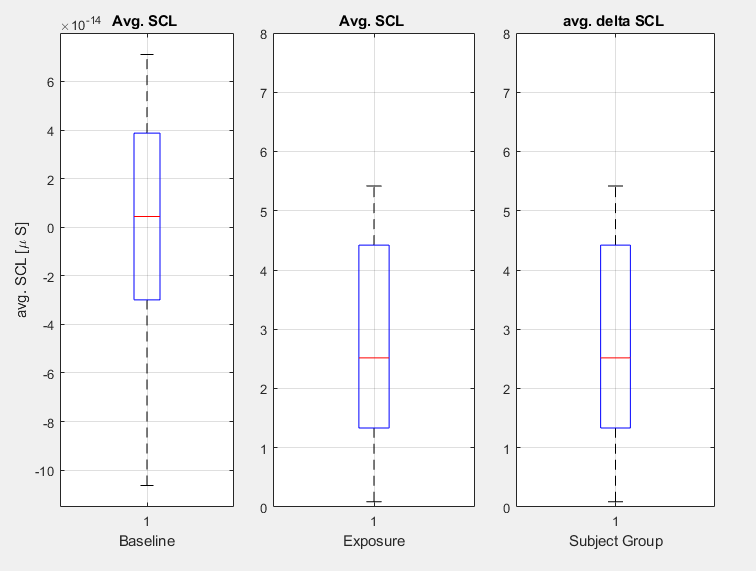
\includegraphics[width=1\textwidth]{images/avgSCL.png}
\caption{Boxplot comparison of the average SCL in subject's baseline (left) and exposure measurement (middle) as well as the average difference in the SCL of the two measurements (right).}
\label{SCLbpImg}
\end{figure}

\newpage
In figure \ref{SCLbpImg} the peak interval distributions of each subject were illustrated in the form of a boxplot for both the baseline and the exposure measurement. The median RR interval is indicated by a red, horizontal line inside the box. The lower and the upper quartile are displayed by the lower and upper edge of the box, respectively. Minimum and maximum value of the peak interval sample are indicated by the endpoints of the, so called,  whiskers (outliers are marked as red +).

\begin{figure}[h]
\centering
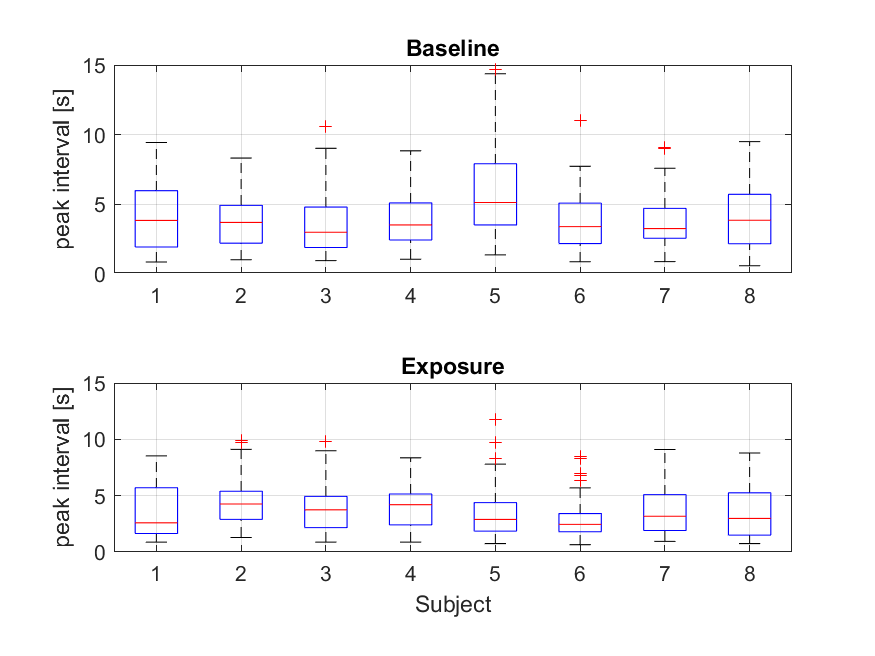
\includegraphics[width=1\textwidth]{images/EDApid.png}
\caption{Boxplot comparison of the peak interval distribution of subject's baseline and exposure EDA measurement.}
\label{SCLbpImg}
\end{figure}

\newpage
An example of an alternative way to illustrate the peak interval distribution is shown in figure \ref{SCLbpImg}. We have created histograms for each subject indicating the frequency of the measured peak intervals. 

\begin{figure}[h]
\centering
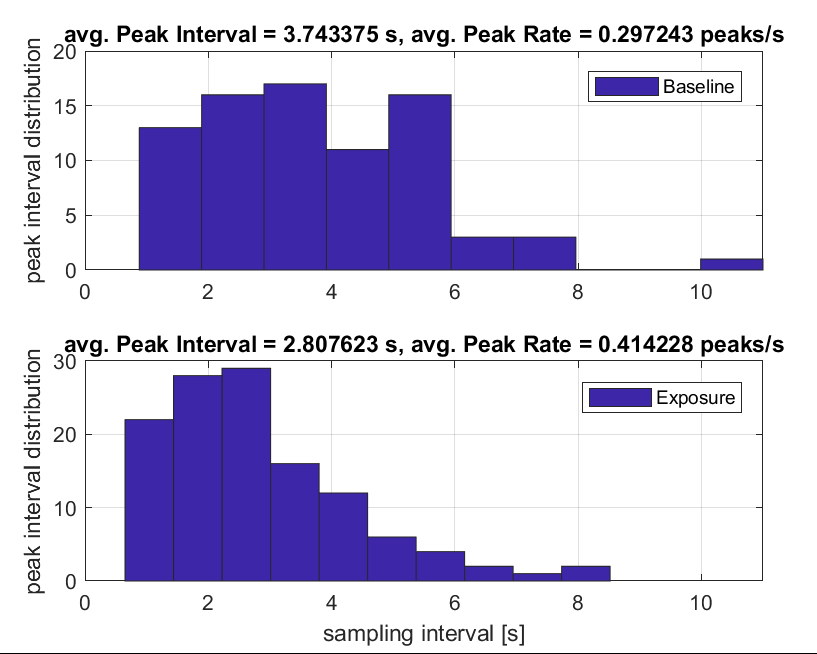
\includegraphics[width=1\textwidth]{images/EDAhisto.png}
\caption{Histogram, illustrating the peak interval distribution of a subject's baseline and exposure EDA measurement.}
\label{EDAhistoImg}
\end{figure}

\newpage
\section{Electrocardiogram}
According to the illustration of EDA, the RR intervals of all subjects are presented in similar fashion in figure \ref{ECGbpImg}. As well as the individual RR distribution in figure \ref{ECGhistoImg}.

\begin{figure}[h]
\centering
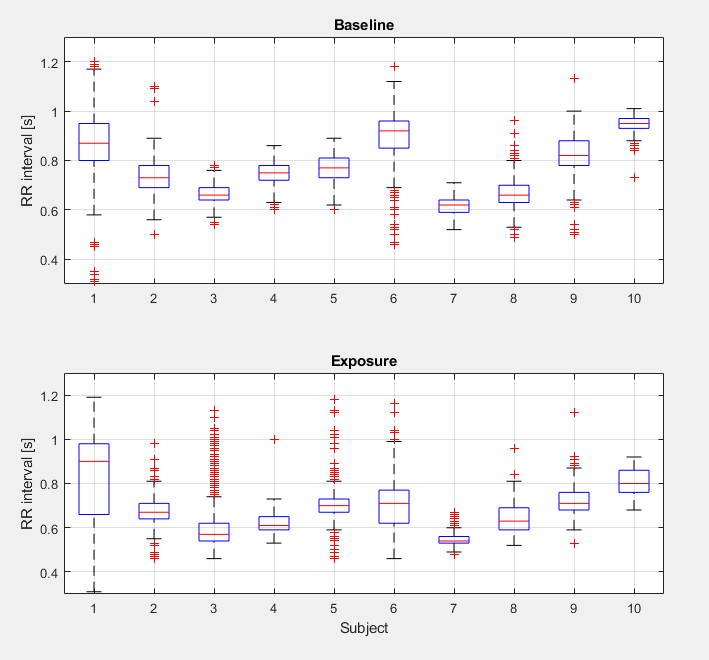
\includegraphics[width=1\textwidth]{images/ECGRRp.png}
\caption{Boxplot comparison of the RR interval distribution of subject's baseline and exposure ECG measurement.}
\label{ECGbpImg}
\end{figure}


\begin{figure}[h]
\centering
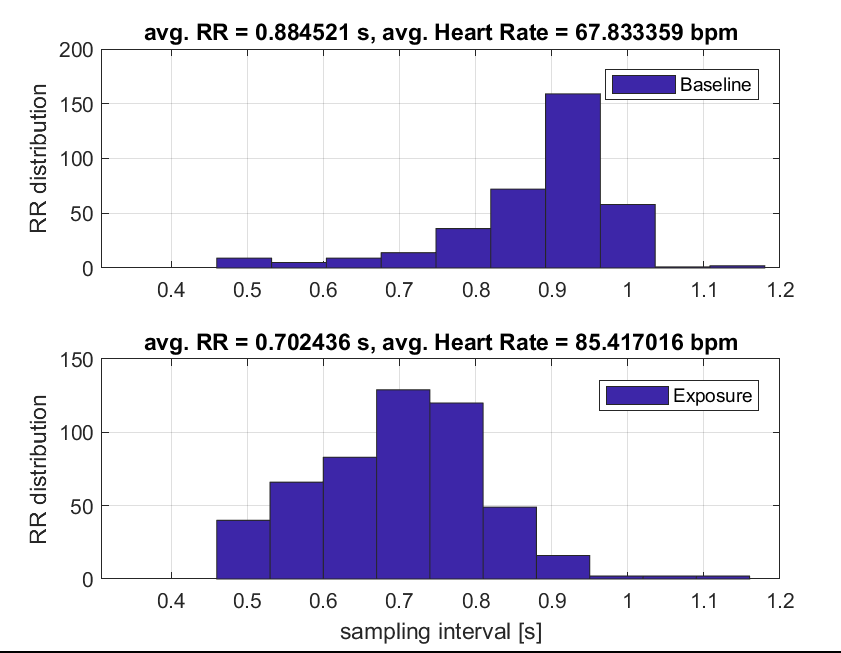
\includegraphics[width=1\textwidth]{images/ECGhisto.png}
\caption{Histogram, illustrating the RR interval distribution of a subject's baseline and exposure ECG measurement.}
\label{ECGhistoImg}
\end{figure}

\newpage
\begin{landscape}
\section{Statistical Results}

\begin{table}[h]
\centering
\caption{Results: Shapiro Wilk test}
\begin{tabular}{|c|c|c|c|c|c|c|c|}
\hline
sample x & n & $\alpha$ & W & $W_{critical}$ & $\bar{x}$ & $a_{i}$ & H\\
\hline
EDA BL & 8 & 0.05 &  0.6621 & 0.818 & 4.1107 & 0.6052 0.3164 0.1743 0.0561 & 1\\
\hline
EDA EP & 8 & 0.05 &  0.8318 & 0.818 & 4.0032 & 0.6052 0.3164 0.1743 0.0561 & 0\\
\hline
SCL BL & 8 & 0.05 &  0.8476 & 0.818 & -1.0882e-15 & 0.6052 0.3164 0.1743 0.0561 & 0\\
\hline
SCL EP & 8 & 0.05 &  0.9511 & 0.818 & 3.3930 & 0.6052 0.3164 0.1743 0.0561 & 0\\
\hline
ECG BL & 10 & 0.05 & 0.9596 & 0.842 & 0.7720 & 0.5739 0.3291 0.2141 0.1224 0.0399 & 0\\
\hline
ECG EP & 10 & 0.05 & 0.9650 & 0.842 & 0.6834 & 0.5739 0.3291 0.2141 0.1224 0.0399 & 0\\ 
\hline	
\end{tabular}
\label{shapirowilk}
\end{table}


\thispagestyle{empty}
\clearpage
\end{landscape}

\newpage

\begin{table}[h]
\centering
\caption{Results: two-sample t-test}
\begin{tabular}{|c|c|c|c|c|c|c|c|}
\hline
sample x & n & $\alpha$ & df & $V_{out}$ & d & t & H\\
\hline
EDA  & 8 & 0.05 &  7 & 1.895 & 0.1074 & 0.2175 & 0\\
\hline
SCL  & 8 & 0.05 &  7 & 1.895 & 3.3930 & 2.9112 & 1\\
\hline
ECG  & 10 & 0.05 & 9 & 1.833 & 0.0886 & 5.8845 & 1\\
\hline	
\end{tabular}
\label{ttest}
\end{table}

\begin{table}[h]
\centering
\caption{Results: effect size test}
\begin{tabular}{|c|c|c|c|c|c|c|c|}
\hline
sample 1& sample 2 & n & mean 1 & mean 2 & $\sigma$ & d & r\\
\hline
EDA EP & EDA BL & 8 & 4.0032 & 4.1107  & 0.9150  & 0.1174 & 0.0073 \\
\hline
SCL BL & SCL EP & 8 & -1.0882e-15 &  3.3930 & 2.3310 & 1.4556 & 0.0906 \\
\hline
ECG EP & ECG BL & 10 & 0.6834 & 0.7720 & 0.0983 & 0.9010 & 0.0450 \\
\hline	
\end{tabular}
\label{effecttest}
\end{table}
